\documentclass{article}
\usepackage[margin=0.5in]{geometry}
\usepackage{graphicx}
\usepackage{amsmath}
\usepackage{listings}
\usepackage{xcolor}
\usepackage{hyperref}

\definecolor{codegreen}{rgb}{0,0.6,0}
\definecolor{codegray}{rgb}{0.5,0.5,0.5}
\definecolor{codepurple}{rgb}{0.58,0,0.82}
\definecolor{backcolour}{rgb}{0.95,0.95,0.92}

\lstdefinestyle{mystyle}{
    backgroundcolor=\color{backcolour},   
    commentstyle=\color{codegreen},
    keywordstyle=\color{magenta},
    numberstyle=\tiny\color{codegray},
    stringstyle=\color{codepurple},
    basicstyle=\ttfamily\footnotesize,
    breakatwhitespace=false,         
    breaklines=true,                 
    captionpos=b,                    
    keepspaces=true,                 
    numbers=left,                    
    numbersep=5pt,                  
    showspaces=false,                
    showstringspaces=false,
    showtabs=false,                  
    tabsize=2
}

\lstset{style=mystyle}

\title{HW 6: Problem 1.1 Analysis}
\author{}
\date{}

\begin{document}
\maketitle

\section*{Problem 1.1: Strategic Network Formation}

\subsection*{Part 1: Undirected Graph with Indicator Payoffs (Linear Model)}
In the undirected model with indicator payoffs (referred to as the ``Linear Model''), both participants of an edge pay the cost $c$ because an edge $\{i,j\}$ increases both $|N_i|$ and $|N_j|$. The benefit of reaching another node does not decay with distance; it is simply $1$ if a path exists. As seen in the code listing in Appendix \ref{sec:code}, we simulate these conditions starting from four distinct initial graph topologies: Empty, Complete, Star, and Cycle graphs.

\begin{itemize}
    \item \textbf{Regime $c < 1$:} We simulated $c=0.5$. The equilibrium reached from all initial states is a tree (8 edges for 9 nodes), which perfectly connects all nodes without any redundant edges. There does not appear to be a \textit{unique} equilibrium graph topology (any spanning tree is an equilibrium because removing an edge breaks the component and losing $\ge 1$ reachability is worse than saving $c=0.5$, while adding an edge yields 0 additional reachability for cost $c$). The resulting trees are highly efficient since they maximize reachability at the minimum possible total edge cost. The total social welfare is mathematically $\Pi(\text{Tree}) = \sum_i (n-1) - 2c \cdot |E| = n(n-1) - 2c(n-1)$. Since any spanning tree (including a star graph) has exactly $|E| = n-1$ edges and $\sum_i (n-1)$ reachability, they all yield the exact same mathematically optimal social welfare of $72 - 8 = 64$. A star is functionally equivalent to a line or any other tree in this specific non-decaying indicator payoff model.
    \item \textbf{Regime $1 < c < n-1$:} We simulated $c=4.0$. From all starting configurations (Empty, Complete, Star, Cycle), the simulation converges to the \textit{empty graph} (0 edges). This is a unique equilibrium because any terminal node (a node with degree 1) pays $c > 1$ to maintain its single edge, but only gains a direct benefit of $1$ from connecting to its neighbor. Even if that neighbor provides transitive reachability to the rest of the network, the terminal node's net marginal benefit for that edge is at most $1 + (n-2) = n-1$. However, the hub node connecting it must also pay $c > 1$ for that specific edge. Since the hub node is already connected to the rest of the network, that specific edge to the terminal node only provides a marginal reachability benefit of exactly $1$. Since $c > 1$, the hub node will strictly prefer to sever the tie ($\Delta\text{Payoff} = c - 1 > 0$), causing the network to systematically unravel from the leaves inward until 0 edges remain. It is severely inefficient. For instance, a centralized star topology would have a socially optimal net positive welfare of $\Pi(\text{Star}) = n(n-1) - 2c(n-1) = 72 - 64 = 8$, but the empty graph leaves us at $\Pi(\text{Empty}) = 0$.
    \item \textbf{Regime $c > n-1$:} We simulated $c=10.0$. The unique equilibrium is the \textit{empty graph}. Because $c > 8$, the maximum possible benefit of playing an edge (reaching all 8 other nodes) is still strictly less than the cost of a single edge ($c=10$). The empty network is efficient in this regime because the maximum conceivable system-wide benefit of an edge (a cycle yielding $2(n-1)$ to the participants and perhaps some transitive benefit to others) is strictly outweighed by the direct costs. Formally, for any network $G$, $\Pi(G) \le n(n-1) - 2c \cdot |E| < 0$ since $c > n-1$ means $2c > 2(n-1) \ge n$ (for $n>2$). Thus $\Pi(\text{Empty}) = 0$ is optimal.
\end{itemize}

\begin{figure}[ht]
    \centering
    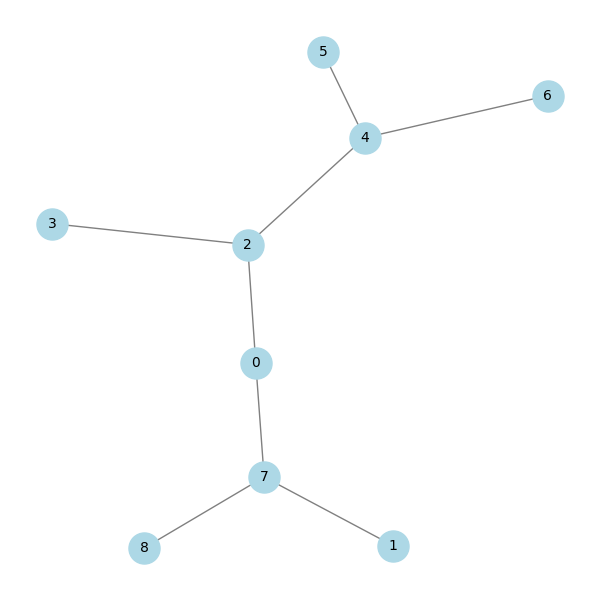
\includegraphics[width=0.5\textwidth]{figs/undirected_linear_c_lt_1_Empty.png}
    \caption{Equilibrium for Undirected Linear ($c < 1$). The network efficiently connects all nodes via a tree without any redundant edges.}
    \label{fig:undir_linear_lt_1}
\end{figure}

As shown in Figure \ref{fig:undir_linear_lt_1}, the equilibrium topography efficiently links every node.

\subsection*{Part 2: Directed Graph with Indicator Payoffs (Linear Model)}
In the directed setting, nodes only pay for their outgoing edges, resolving the bilateral cost-sharing resistance seen in the undirected case. However, unlike undirected edges where a single link $\{A, B\}$ provides mutual two-way access, a directed edge $(A, B)$ only provides $A$ access to $B$, not vice-versa. This implies that a tree topology ($n-1$ edges), which perfectly connects an undirected graph, cannot provide full reachability in a directed graph because there is no path back to the roots. The minimal structure to achieve full global reachability (strong connectivity) is a directed cycle ($n$ edges).

\begin{itemize}
    \item \textbf{Regime $c < 1$:} We simulated $c=0.5$. Because $c < 1$, any unreached node provides $1$ benefit for only $c$ cost, prompting nodes to form links until the graph is strongly connected. A perfect directed cycle (9 edges for 9 nodes) is an efficient equilibrium with a maximal social welfare of $\Pi(\text{Cycle}) = \sum_i (n-1 - c \cdot 1) = n(n-1 - c) = 9(8-0.5) = 67.5$. The cycle is the most efficient topology because it provides every node full indicator reachability ($+8$) using the absolute mathematical minimum number of directed edges ($n=9$). This shifts the optimal structure from an $n-1$ edge tree in Part 1 to an $n$ edge cycle in Part 2, a direct consequence of the one-way nature of directed traversal. While the simulation sometimes converged to local Nash Equilibria with slightly more non-redundant edges depending on initialization, the cyclical motif remains paramount for reachability. 
    \item \textbf{Regime $1 < c < n-1$:} We simulated $c=4.0$. The equilibria are deeply dependent on the initialization. If started from an empty graph or an inward star, no node wants to pay $c=4.0$ to reach just 1 node, so the \textit{empty graph} remains a stable equilibrium (inefficient, $\Pi = 0$). Conversely, if initialized as a complete graph, outward star, or cycle, the network trims down precisely to a \textit{directed cycle} (9 edges). A cycle is a Nash Equilibrium because each node pays $c=4.0$ for $1$ outgoing edge but achieves a reachability of $8 \times 1 = 8$, netting $+4.0$. The cycle is an efficient topology here, achieving the maximum welfare $\Pi = n(n-1-c) = 36$.
    \item \textbf{Regime $c > n-1$:} We simulated $c=10.0$. As in the undirected case, the cost of a single edge exceeds the absolute maximum reachability benefit of $n-1 = 8$. Thus, all nodes rapidly sever all outgoing edges, leaving the \textit{empty graph} as the unique and efficient equilibrium ($\Pi=0$).
\end{itemize}

\begin{figure}[ht]
    \centering
    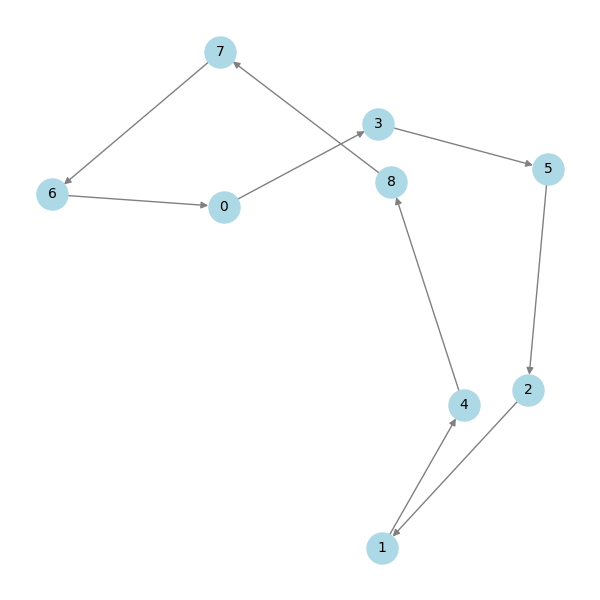
\includegraphics[width=0.5\textwidth]{figs/directed_linear_1_lt_c_lt_n-1_Complete.png}
    \caption{Equilibrium for Directed Linear ($1 < c < n-1$) starting from a dense graph. The result trims precisely to an efficient directed cycle.}
    \label{fig:dir_linear_cycle}
\end{figure}

Figure \ref{fig:dir_linear_cycle} visualizes this cyclical stability.

\subsection*{Part 3: Undirected Graph with Distance Payoffs (Connections Model)}
In the connections model, the benefit explicitly decays with distance ($\delta = 0.5$).
\begin{itemize}
    \item \textbf{Regime $c < \delta - \delta^2$:} We tested $c=0.1$. As seen in Figure \ref{fig:undir_conn_small}, the simulation instantly converges from any initialization to the \textit{complete graph} (36 edges). Since $c < 0.25$, any node prefers adding a direct edge to another node rather than having an indirect path of distance 2 or more, as the gain ($\delta - \delta^2 = 0.25$) exceeds the cost $c$. Thus, it is the unique equilibrium and is efficient. The welfare mathematically is $\Pi(\text{Complete}) = n(n-1)(\delta - c) = 9(8)(0.5 - 0.1) = 28.8$.
    \item \textbf{Regime $\delta - \delta^2 < c < \delta + (n/2 - 1)\delta^2$:} We tested $c=0.8$. Starting from an empty graph (where no nodes share any edges), the simulation trivially terminates because adding the very first edge costs $0.8$ but only provides a direct marginal benefit of $\delta=0.5$. This empty equilibrium is rigorously inefficient ($\Pi=0$). 
    
    However, if we initialize the simulation from dense, highly-connected topologies (such as the Complete graph, Star graph, or Cycle graph), the simulation enters continuous cyclic behaviors (plotted in Figure \ref{fig:undir_conn_conv}). This instability occurs because nodes now disagree on the network's value depending on their algorithmic structural position. Peripheral nodes strictly benefit from finding cheap, short paths through central ``hubs'', so they aggressively desire to form or maintain links. But the central hub itself pays immense, compounding link costs (-0.8 per edge) without receiving equivalent distance payoffs (since it already had short paths to most nodes). As a result, the hub inevitably severs its ties to save cost. This fractures the network, raising distances for the peripheral nodes, who then frantically try to build new edges to reconnect—causing the cycle to endlessly repeat without finding a stable Nash Equilibrium. This regime highlights a stark conflict between Nash equilibrium stability and social welfare: the socially optimum topology (the Star graph) has a strongly positive efficiency ($\Pi = 8(2(0.5) - 2(0.8)) + 56(0.5^2) = -4.8 + 14 = 9.2$), but no individual hub node will stably shoulder the personal cost to maintain it. Consequently, the network is either trapped at the $0$ efficiency empty state or forced to endlessly cycle through suboptimal, transient inefficiencies.
    \item \textbf{Regime $c > \delta + (n/2 - 1)\delta^2$:} We tested $c=2.0$. It firmly resolves back to the \textit{empty graph} from almost all common starting points. Edge costs systematically overpower proximity rewards on all structural vectors ($2.0 > 0.5 + (3.5)*0.25 = 1.375$), so nodes aggressively drop edges. The empty graph is uniquely efficient $\Pi=0$ and acts as the predominant strong stable equilibrium here.
\end{itemize}

\begin{figure}[ht]
    \centering
    \begin{minipage}{0.48\textwidth}
        \centering
        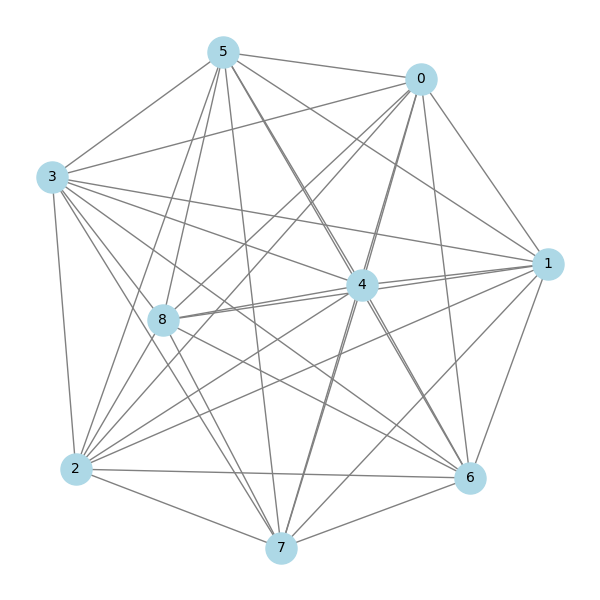
\includegraphics[width=\textwidth]{figs/undirected_conn_c_small_Empty.png}
        \caption{Equilibrium for Undirected Connections ($c < \delta - \delta^2$). Penalizing indirect paths quickly settles it into a complete graph.}
        \label{fig:undir_conn_small}
    \end{minipage}\hfill
    \begin{minipage}{0.48\textwidth}
        \centering
        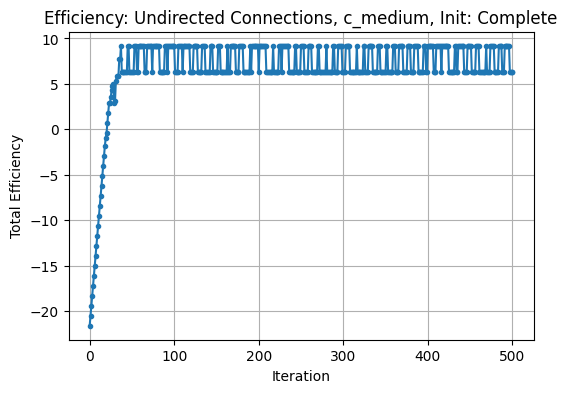
\includegraphics[width=\textwidth]{figs/conv_undirected_conn_c_medium_Complete.png}
        \caption{Efficiency convergence for Undirected Connections ($c=0.8$) initialized from Complete graph. The system cycles continuously without a stable equilibrium.}
        \label{fig:undir_conn_conv}
    \end{minipage}
\end{figure}

Figure \ref{fig:undir_conn_small} shows the uniform clustering of edges when direct distances are heavily rewarded, while Figure \ref{fig:undir_conn_conv} demonstrates the cyclic instability in the intermediate cost regime.

\newpage
\section*{Problem 1.2: Escaping the Cursed Maze}

\subsection*{1. Why BFS/DFS Fails}
Standard graph search algorithms like Depth-First Search (DFS) or Breadth-First Search (BFS) rely on a deterministic transition framework: if a node attempts to move North, it implicitly trusts that the resulting state will strictly be the room to the North. However, the cursed maze introduces a $p=0.20$ probability of ``slipping'' on a conveyor belt, forcing the agent into a random adjacent room. This stochastic transition matrix destroys the absolute viability of static paths. Even if BFS finds the absolute shortest sequence of cardinal moves to an exit, it cannot guarantee that sequence will actually be executed. Crucially, algorithms like BFS fail to internalize risk: a shortest path that skirts tightly along the edge of multiple snake rooms is astronomically dangerous under a $20\%$ slip rate, but BFS cannot distinguish this probabilistic danger from a safe open corridor as long as the step count is identical.

\subsection*{2. TD(0) Learning and Escaping}
To successfully navigate the maze, we modeled the problem as Reinforcement Learning over a Markov Decision Process, specifically utilizing a Temporal Difference TD(0) value update rule. We learned the state value function $V(s)$ by exploring the maze for 998 episodes using an $\varepsilon$-greedy policy to balance exploiting known safe paths and exploring unknown areas.

\textbf{Hyperparameters Configured:}
\begin{itemize}
    \item \textbf{Learning Rate} $\alpha = 0.5$: A moderate learning rate to quickly backpropagate terminal signals while smoothing out the noise from stochastic collisions.
    \item \textbf{Exploration} $\varepsilon$: Decayed exponentially from $1.0$ down to $0.05$ over the 998 episodes using a $0.995$ multiplier per episode, ensuring broad early exploration that gradually settles into confident exploitation.
    \item \textbf{Rewards}: Snakes were initialized and permanently fixed at $-100.0$, escapes fixed at $+100.0$. Standard, unexplored square rooms began at $0.0$.
\end{itemize}

During our empirical test consisting of $1000$ iterations with a purely greedy policy ($\varepsilon = 0$), the agent successfully escaped the maze \textbf{1000 out of 1000} times, achieving a 100\% survival rate. Because the agent directly learned $V(s)$ from stochastic experience, it implicitly learned to heavily discount the values of rooms directly physically adjacent to snakes—punishing the areas where slipping would be lethal. This phenomenon is directly supported by Figure \ref{fig:maze_values}, which shows distinct low-value suppression zones surrounded by the 'S' rooms. Thus, the greedy policy naturally prefers longer, safer corridors over dangerous shortcuts.

\begin{figure}[ht]
    \centering
    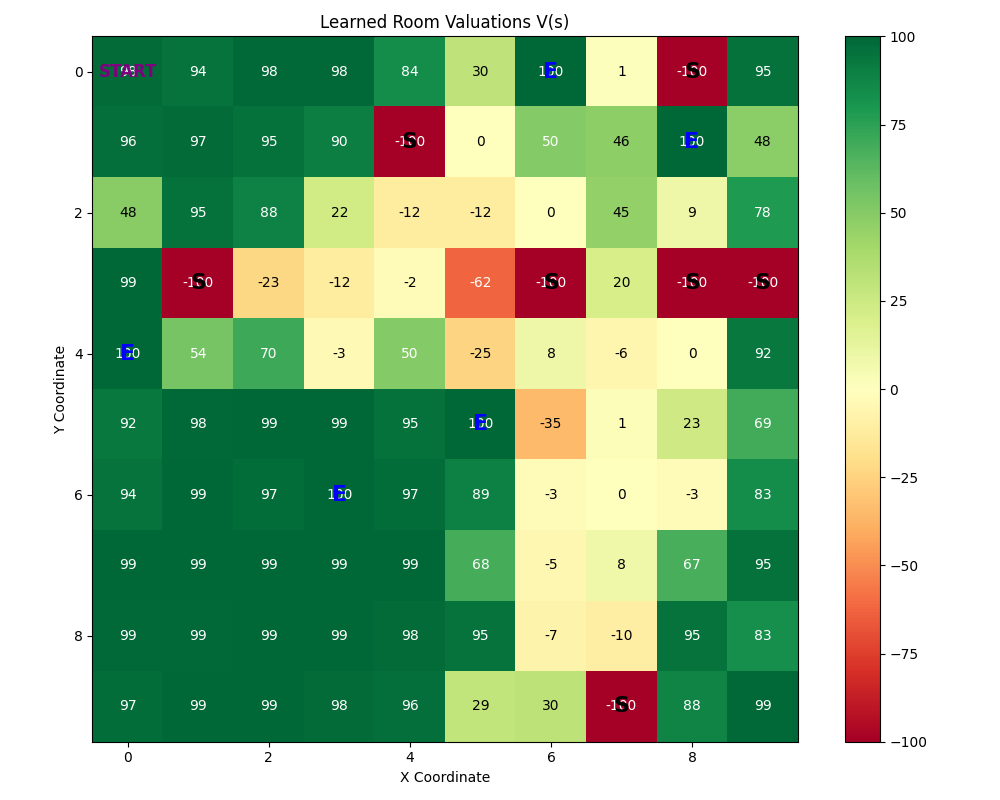
\includegraphics[width=0.6\textwidth]{figs/maze_learned_values.png}
    \caption{The converged $V(s)$ state-value grid after 998 episodes. Safest, most attractive rooms radiate outward from the escapes (E), while regions bordering snakes (S) are heavily suppressed.}
    \label{fig:maze_values}
\end{figure}

The fully converged state-valuation grid $V(s)$ that drives the optimal policy is plotted in Figure \ref{fig:maze_values}. The complete Python implementation for learning and solving the maze (\texttt{solve\_maze.py}) is provided in Appendix \ref{sec:maze_code}.

\newpage
\section*{Problem 2: Theory}

\subsection*{2.1 Routing Games with Tolls}

We are given a routing game with $N$ players, each with traffic $r_i = 1$. The original link cost function is $c_e(x)$ and the original objective function is the social cost:
$$ W(f) = \sum_{e \in E} f_e c_e(f_e) $$
where $f_e$ is the total traffic (number of players) on edge $e$. We introduce a new cost function with a toll:
$$ c^*_e(x) = c_e(x) + (x-1)\left(c_e(x) - c_e(x-1)\right) $$
We must prove that the flow $f^*$ that minimizes the original social cost $W(f)$ is a pure Nash Equilibrium for the new game with costs $c^*_e(x)$. 

To prove this, we construct the exact potential function $\Phi^*(f)$ for the new game. For any routing game with integer flows and edge costs $c^*_e(x)$, the standard Rosenthal potential function given is:
$$ \Phi^*(f) = \sum_{e \in E} \sum_{x=1}^{f_e} c^*_e(x) $$

Let us substitute the new cost function $c^*_e(x)$ into this potential function and simplify the inner sum for a single edge $e$:
\begin{align*}
\sum_{x=1}^{f_e} c^*_e(x) &= \sum_{x=1}^{f_e} \left[ c_e(x) + (x-1)c_e(x) - (x-1)c_e(x-1) \right] \\
&= \sum_{x=1}^{f_e} \left[ x c_e(x) - (x-1)c_e(x-1) \right]
\end{align*}

Notice that this inner sum is a perfect telescoping series! Let $g_e(x) = x c_e(x)$. The sum becomes:
\begin{align*}
\sum_{x=1}^{f_e} \left[ g_e(x) - g_e(x-1) \right] &= (g_e(1) - g_e(0)) + (g_e(2) - g_e(1)) + \dots + (g_e(f_e) - g_e(f_e-1)) \\
&= g_e(f_e) - g_e(0)
\end{align*}

Since $g_e(0) = 0 \cdot c_e(0) = 0$, we simply have:
$$ \sum_{x=1}^{f_e} c^*_e(x) = f_e c_e(f_e) $$

Substituting this back into the full potential function $\Phi^*(f)$:
$$ \Phi^*(f) = \sum_{e \in E} f_e c_e(f_e) = W(f) $$

We have shown that the exact potential function $\Phi^*(f)$ of the new game with tolls is mathematically identical to the social cost objective function $W(f)$ of the original game. 

By the fundamental property of potential games, any pure Nash Equilibrium is a local minimum of the potential function. More importantly, the global minimum of the potential function is guaranteed to be a pure Nash Equilibrium. Since $f^*$ is the optimal strategy that globally minimizes $W(f)$, and $W(f) = \Phi^*(f)$, $f^*$ globally minimizes the potential function of the new game. Therefore, $f^*$ must be a Nash Equilibrium for the new game. 

\newpage
\appendix
\section{Code Listing}
\label{sec:code}
\lstinputlisting[language=Python]{../code/simulate_networks.py}

\subsection*{solve\_maze.py}
\label{sec:maze_code}
\lstinputlisting[language=Python]{../code/solve_maze.py}

\end{document}
